\documentclass[a4paper, 11pt]{article}
\newcommand{\systemTitle}{NINSHIKI}
\usepackage[bottom]{footmisc}
\usepackage{minted}
\usepackage{graphicx}
\usepackage{fontspec}
\usepackage{hyperref}
\usepackage{rotating}
\usepackage{epstopdf}
\usepackage{appendix}
\usepackage{tabto}
\usepackage{float}
    \setmainfont[Path = ./MavenPro/,
 				  Extension = .ttf,
 				  UprightFont = *-Regular,
 				  BoldFont = *-Bold]
                  {MavenPro}
    \setsansfont[Path = ./NunitoSans/,
 				  Extension = .ttf,
 				  UprightFont = *-Light,
 				  BoldFont = *-SemiBold,
                  ItalicFont = *-LightItalic]
                  {NunitoSans}
\usepackage{fancyhdr}
    \pagestyle{fancy}
    \fancyhf{}
    \rhead{Software Sharks}
    \setlength{\headheight}{16pt} 
    \lhead{\systemTitle{} - Testing Manual}
    \rfoot{Page \thepage}


\title{Testing Manual}
\author{Software Sharks}
\date{September 2018}

\begin{document}

%----------------------------------------------------------------------------------------
%	TITLE PAGE
%----------------------------------------------------------------------------------------
\begin{titlepage}
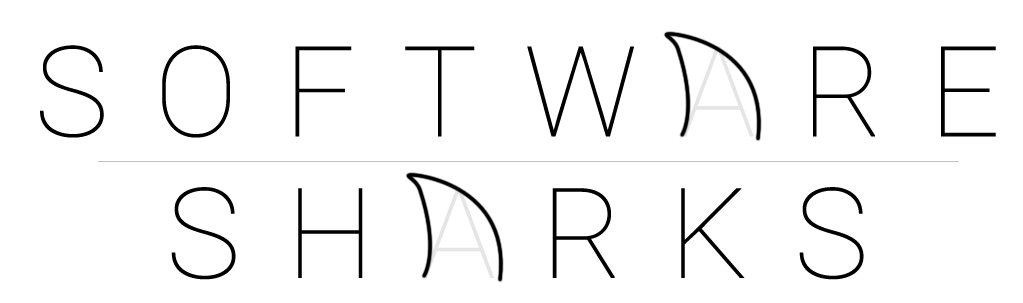
\includegraphics[width=0.5\linewidth]{images/sslogo.png}
	\centering
	
    \scshape
    \sffamily
	
	\vspace*{\baselineskip}
	
	\rule{\textwidth}{3pt}
	
	\vspace{0.75\baselineskip}
	
	\textrm{\LARGE \textbf{Testing Manual} \\ for\\ \systemTitle{}\\ \small Version 1.0.0 - Demo \#5 Draft\\}
	
	\vspace{0.75\baselineskip}
	
	\rule{\textwidth}{3pt} 
	
	\vspace{2\baselineskip}
	
	A guide to the testing process used in the development of the Ninshiki system, including the test procedures, tools and frameworks, as well as the functional test cases and the history of various functional and nonfunctional requirement testing.\\
	
	\vspace*{3\baselineskip}
	
	Compiled By
	
	\vspace{0.5\baselineskip}
	
    \textsf{\large
    \textrm{\textbf{The Software Sharks Team}} \\
    \small 
    Coetzer MJ \\
    Bester TJ \\
    Orrie O \\
    Lew J \\
    Matodzi MC \\
    } 
	
	\vspace{0.5\baselineskip}
	
	\textit{ Department of Computer Science \\ The University of Pretoria}
	
    \vfill
    \includegraphics[width=0.5\linewidth]{images/uplogo.png}
    \vfill
    For
	
	\vspace{0.5\baselineskip}
	
    \textsf{\large
    \textrm{\textbf{Bramhope International School of Innovation}} \\
    } 

\end{titlepage}

\pagebreak

%----------------------------------------------------------------------------------------
%	COPYRIGHT PAGE
%----------------------------------------------------------------------------------------

\newpage
~\vfill
\thispagestyle{empty}

\noindent COS 301 Team: Software Sharks\\ 

\noindent \textsc{Department of Computer Science, University of Pretoria}\\

\noindent \textsc{https://github.com/OrishaOrrie/SoftwareSharks}\\ % URL

\noindent This testing manual document was drafted under the supervision of involved lecturers according to the assessment guidelines of the final year Computer Science module: COS 301 - Software Engineering, presented by the Department of Computer Science in the faculty of Engineering, Built Environment and Information Technology at the University of Pretoria during the first and second semesters of the year 2018. \\ \\

\noindent \textit{First release, September 2018} % Edition date

\pagebreak

%----------------------------------------------------------------------------------------
%	Table of Contents
%----------------------------------------------------------------------------------------
\tableofcontents

\pagebreak


%----------------------------------------------------------------------------------------
%	Introduction
%----------------------------------------------------------------------------------------
\section{Introduction}
This is a document describing all the test procedures used throughout the development of the Ninshiki system. First, the specific testing procedures will be discussed for each functional subsystem, as well as for each nonfunctional requirements. Then, the tools and frameworks used to carry out these procedures will be elaborated. Thirdly, the test cases/functions used to check that each requirement is met will be defined. Finally, the history and location of test logs of each subsystem will be discussed.

\section{Testing Process}
The following section discusses the processes undertaken to test the various functional and nonfunctional requirements of each subsystem. The details of each test is discussed, including the method and frequency of each test.

    \subsection{Functional}
    
        \subsubsection{General Testing Process}
        The development of the system follows the principles of Test-Driven Development. The general testing process is as follows:\\
        \begin{enumerate}
            \item For each use case, a test function is written that acts as a user completing a task.
            \item Initially, all test functions fail. If they don’t, they are rewritten so that they fail.
            \item Starting from the highest priority use cases, the functional classes and programs that solve each use case are implemented, so that the respective test functions succeed.
            \item This is repeated until all functions are implemented, all use cases are solved, and all test functions pass successfully.
        \end{enumerate}
        This procedure is followed when writing test functions and test cases for each subsystem.
        
        \subsubsection{Application Testing Process}
        \paragraph{}
        Since the web and mobile application is built using the Angular framework (the Ionic framework used for mobile is based on Angular), the codebase for each subsystem is very similar, differing only in the way images are captured or selected from gallery. For this reason, this section will encapsulate the functional testing procedure for both subsystems.
        \paragraph{}
        The functionality of the applications are tested against the system use cases, with one set of functions written for each use case. These test functions comprise the end-to-end tests, and are run using Protractor and written with Jasmine. The test cases are described in section 3. Complete, automated end-to-end tests are performed after the addition of a new feature or after the completion of a change to the app.
        \paragraph{}
        Each use case is also assigned to a component of the app. This means that each component needs to be unit tested. Unit testing is done to ensure that the internal structure of the application serves its purpose, handles errors correctly, and has no flaws. A set of unit test functions are written for each component in an isolated manner. These tests are run via Karma and written with Jasmine. Automated unit tests are run after any changes are made to a single component.
        \paragraph{}
        The full set of unit tests and end-to-end tests are run when a new set of code is pushed to the GitHub repository master branch. This is done automatically via Travis CI, which executes a script on a remote PC and sends a report to the developers upon completion. This ensures that both kinds of tests are done for the application without the need for personal resources. It also prevents faulty software from being deployed.
    
    \subsection{Non-Functional}
        \subsubsection{Performance}
        This section describes the process of testing the performance of the various subsystems.
        
            \paragraph{Web App Performance Testing}
            The performance of the web application is tested to check whether the response time is fast enough so that the user does not get frustrated, but rather can use the web app efficiently. Two tools are used to test the performance of the web app: the one runs tests on the local browser, the other runs tests in a hosted environment. The second tool provides a generally more accurate and consistent report, since local testing can be influenced by things such as anti-virus scanners, browser extensions, etc.
            \paragraph{}
            Google Lighthouse Audit is used to test response time locally. The Performance category of the audit provides different metrics such as first meaningful paint, first CPU idle, and time to interactive. All of these metrics are used in conjunction to determine whether the overall site response time meets the performance requirements. If the report indicates that at least four out of six metrics are good (green), then the performance test has been passed.
            \paragraph{}
            WebPagetest is used to test response time from a hosted environment. It runs performance tests much like Lighthouse, but the location, browser, and bandwidth quality of the test can be specified. WebPagetest also specifies the performance details of the test in more depth. It also provides grades that indicate whether a set of metrics is at a good level. If the report indicates that the first byte time received a “B” or higher, then the performance test has been passed.
            \paragraph{}
            Both tools are used to perform tests each time the web app is deployed and hosted on Firebase, so that it can be tested as if it were an actual website. The Lighthouse Audit is part of the Travis continuous integration script.
            \paragraph{Mobile App Performance Testing}
            Much like the web app, the response time of operations in the mobile app needs to be tested to see that it aids, not deters usability. Two different tools are also used for the same purpose: one tool is used to test performance locally and the other is used to test in a hosted environment.
            \paragraph{}
            Lighthouse is used once again to test the performance of the mobile app locally. This is possible because the app is built with Ionic, which uses the web-based Angular framework. Therefore, the app can be treated as a website before it is packaged as a native mobile app. Testing is done the same way as with the web app Lighthouse testing. The Lighthouse Audit is conducted every time the app is to be deployed, just before the app is packaged into a native app.
            \paragraph{}
            Once the packaged native app is produced (as an APK file), a second tool called Firebase Test Lab is used to check app performance on eight different kinds of Android phones, with different OS versions and different screen sizes. The Test Lab produces various performance-related time-series graphs. These graphs indicate how RAM and CPU usage vary in different sections of the app. This is useful in optimizing the performance of different operations of the app. These tests are performed every time an APK is built, i.e. every production release.
            \paragraph{}
            Once the app is deployed and used, Firebase collects various analytics related to performance and crashes. The Firebase dashboard displays these performance metrics and crash reports in a neat, easy to read format.
            \paragraph{}
            These three tools are used to ensure that performance requirements are met at three different stages of the app development life-cycle.
        
        \subsubsection{Security}
        % TO-DO
        
        \subsubsection{User Interface}
            \paragraph{}
            The user interface is one of the most important aspects of an application. The look and feel is what will make users want to use the application. Since the application has been created for everyday use by warehouse workers, it should be simple to use with neutral colours.
            \paragraph{}
            The two main functions are the image prediction and weight analysis since those what the workers will be using the most often. Both of these have a very simple interface as well as instructions on how to use them in order to make the interface even simpler.
            \paragraph{}
            In order to test these features, usability tests were done throughout the life-cycle of the project. In this usability test, a few aspects such as efficiency, satisfaction as well as productivity were tested.
            
        \subsubsection{Image Prediction}
            \paragraph{}
            This section describes the testing process for the image classifier model. This tests the accuracy of a model by feeding it a set of test images, at least one for each class, and comparing the predicted label of that image to the actual class label. Correct predictions are ones that predict the actual class as the most likely. Top 8 predictions are ones that predict the actual class as within the top 8 most likely classes.
            \paragraph{}
            A Python script is used to run the entire set of predictions, while the results are recorded manually in a spreadsheet. This process is completed every time a new model is built.

\section{Testing Tools}
Various testing frameworks and tools are used to automate unit and end-to-end tests, as well as visualize the tests for non-functional requirements. This section describes each tool used, as well how they are configured and why they were chosen.

    \subsection{Functional}
    This section describes the tools used when testing that the subsystems meet the use cases.
    
        \subsubsection{Application Testing Tools}
        As mentioned in section 1, there are different tools used for each kind of testing. Each tool is described below.
        
            \paragraph{Jasmine}
            Jasmine is a testing framework that allows for test functions to be written in JavaScript/TypeScript that supports Test-Driven Development. Jasmine allows for functions to be written in a low-level, easy-to-understand format. Multiple JavaScript test scripts can be run by a single Jasmine HTML file. The actual test functions for both the unit and end-to-end tests for the mobile and web applications are written using Jasmine. Jasmine test files are setup and configured automatically upon creation of an Angular project. Unit tests for each component and service can be found in the respective component spec.ts file, which is found in the component folder. They are executed by running the command ‘ng test’.
            \paragraph{}
            Jasmine was selected to write test functions because it is the recommended testing framework for Angular.
            
            \paragraph{Karma}
            Karma is an automated test runner that integrates with Angular and Jasmine. It runs a separate browser with all Jasmine unit tests running. Karma automatically re-runs all Jasmine test functions each time a change is made to the development environment. Karma is also pre-configured upon creation of an Angular project.
            \paragraph{}
            Karma was also selected due to it being the recommended testing tool for Angular. The combination of Jasmine and Karma aids Test-Driven Development, and makes the unit testing process simple and efficient.
            
            \paragraph{Protractor}
            Protractor is an end-to-end testing framework that runs test functions on a real browser automatically. This means that tests are performed as if they were done in a real environment. Protractor makes end-to-end testing easy by automating things such as waiting, as it smartly detects when changes to a page have been made. Protractor can easily be configured with an Angular project and often comes pre-configured.
            \paragraph{}
            Protractor was selected due to its compatibility with Jasmine and Angular in general. It is also useful for end-to-end testing event-driven applications.
            
            \paragraph{Travis CI}
            Travis CI is a continuous integration service that automates integration and deployment processes. Travis executes a script every time a push is made to the Master branch of the GitHub repository. The script may execute commands that assist in various processes such as unit testing, end-to-end testing, and deployment. This script file can be found and edited in the root directory of the repository.
            \paragraph{}
            Travis was selected due to its ability to automatically run the full suite of test cases by executing the appropriate Karma and Protractor commands. It can also be setup so that if no major faults are discovered, it automatically deploys the system (in the case of this project, it would deploy the web app to Firebase for hosting).
            
    \subsection{Non-Functional}
        \subsubsection{Performance}
        
            \paragraph{Google Lighthouse Audit}
            Lighthouse is a tool available as a Node module with a command line interface and as part of Google Chrome browser Developer Tools. It performs an audit on any given website via a URL, and allows for the mobile or desktop version of the website to be tested. The audit produces an HTML report with scores for five different categories, namely: Performance, PWA (Progressive Web App), SEO (Search Engine Optimization), Best Practices, and Accessibility. Not only do these scores give a good indication of the performance of the web app, the report also produces guidelines and optimization tips to help improve each of the five aspects. Lighthouse was selected due to its easy to understand reports, helpful guidelines, and ability to be used with Travis-CI.
            \paragraph{}
            A Lighthouse Audit can be run by entering the Developer Tools on selected browsers, navigating to the Audit tab, and specifying a few preferences. Alternatively, the audit can be run from the command line by using “lighthouse <url>”, provided the Lighthouse npm package is installed.
            
            \paragraph{WebPagetest}
            WebPagetest is a website that performs a performance review on a given website via the URL. The location, bandwidth quality, and browser on which the test is run can be specified, and then the test is performed in that specific environment. The tool produces a detailed report, including waterfall graphs, which help developers understand the process of the website loading onto the user’s browser. The report also gives grades to various performance attributes of the website, so that these attributes can be identified and improved upon. WebPagetest was selected as a tool due to it being recommended by the Lighthouse documentation, and because it produces more consistent and accurate test results than Lighthouse.
            \paragraph{}
            WebPagetest can be accessed from \url{https://www.webpagetest.org/} and simply requires the URL of the website to be input.
            
            \paragraph{Firebase Test Lab}
            Firebase is a platform that provides various services that power up the development and deployment of mobile and web applications, such as performance analysis on live app sessions. One of these services used in this project is called Test Lab, which simply requires an APK to be uploaded in order for a mobile application to be tested. Test Lab automatically runs what it calls Robo tests on real devices, which runs the app, programmatically presses all the buttons on the app in sequence, and produces performance graphs and a video recording of the test. This helps developers understand the performance of the app on various device models. Test Lab was chosen because Firebase was already in use for the deployment of the app, and because it makes performance testing on various device models simple and efficient, without having the need to obtain an infrastructure or find users with different devices.
            \paragraph{}
            Test Lab simply requires a Firebase project to be created and for any APK to be uploaded. The only settings that need to be configured are the number and type of devices that are to run the test.

         \subsubsection{Security}
            \paragraph{In-House Penetration Testing}
            The security of the web application end point was tested via several brief tests, detailed below, aimed at gaining unintended access to files or functions.
            \begin{itemize}
                \item SQLMap: A SQLMap script was run to identify possible injection parameters in malformed URI's
                \item NMap: A NMap script was run against the server to identify possible open ports and unwanted access points
            \end{itemize}
            
            \paragraph{In-depth Results and Conclusions}
            % Busy formatting
        
         \subsubsection{User Interface}
            \paragraph{}
            To test the user interface, Usability testing was done where a Google form was created and a series of questions relating to the user interface were asked. These tests were done on people from different backgrounds and skill levels.
            \paragraph{}
            In order to better the user interface even further, a meeting was held, with a lecturer at the University of Pretoria, who specializes in User interface design as well as User experience. He helped us to properly place different features of both the web app as well as the mobile app in correct places so that users will find it easier to access these features.
            \paragraph{}
            From these results, an analysis was done and changes to the user interface were completes. Once these changes were completed, another usability test was done and this cycle continued throughout the life-cycle of the project.
            
        \subsubsection{Image Prediction}
            No special test tools are used to test the accuracy of a model. The model is tested by running a script that runs the Predict method on each test image.

\pagebreak
\section{Test Cases}
The following section describes the test cases used to check whether each aspect of the requirements are met. The majority of these formal test cases are for the unit and end-to-end test code for the functionality testing.
    
    \subsection{Functional}
    This section describes the individual test functions for each of the use cases. The locations in the GitHub repository for the test cases of each subsystem are also indicated.

        \subsubsection{Application Test Cases}
        The following use cases each have associated end-to-end test functions. These tests are all executed in sequence by running the command ‘ng e2e’ in the ss-imagerec-web folder. The tests functions can be found here:\\
        \url{https://github.com/OrishaOrrie/SoftwareSharks/blob/master/Application\%20Source/ss-imagerec-webapp/e2e/app.e2e-spec.ts}
        
        \begin{enumerate}
            \item Use Case: Capture an Image
                \begin{enumerate}
                    \item Test Function: If the “Webcam” button is clicked, then check if the webcam is opened and check if the video capture is displayed on the page.
                    \item Test Function: If the “File Select” button is clicked, then check if the file explorer has been opened and check if a selected image is displayed on the page.
                \end{enumerate}
            \item Use Case: Submit Image
                \begin{enumerate}
                    \item Test Function: If an image is displayed, then it must have been captured or selected, so check if the “Submit” button is displayed.
                    \item Test Function: If the “Submit” button is clicked, then check if the text on the button changes to “Predicting...”
                \end{enumerate}
            \item Use Case: Receive/View Results
                \begin{enumerate}
                    \item Test Function: If an image has been submitted, then check whether the window scrolls down to the results table.
                    \item Test Function: If an image has been submitted, then check whether entries exist in the results table.
                    \item Test Function: If an image has been submitted, then check whether an entry contains a link that can be clicked, opening a page from the Bramhope catalogue in a new tab.
                \end{enumerate}
            \item Use Case: Weight Analysis
                \begin{enumerate}
                    \item Test Function: If an input field is touched or dirtied, check that the “Item Amount” check is updated dynamically.
                    \item Test Function: If an input field is made blank, check that the status bar is updated to display an appropriate message.
                    \item Test Function: If a negative value is input, check that the status bar is updated to display an appropriate message.
                    \item Test Function: If the input weight for an empty bucket is greater than the input weight for a filled bucket, check that the status bar is updated to display an appropriate message.
                    \item Test Function: If the input tuple for (single\_item, empty\_bucket, filled\_bucket) is (5, 5, 20), check that the status bar is updated to display “Amount of Items: 3”.
                \end{enumerate}
            \item Use Case: Contact Company
                \begin{enumerate}
                    \item Test Function: If an input field is touched or dirtied, then check whether validation is done on the field dynamically.
                    \item Test Function: Check whether invalid email field values are rejected.
                    \item Test Function: If all input fields are valid, then check whether the “Submit” button is enabled.
                    \item Test Function: If the “Submit” button is clicked, then check whether a loading spinner is displayed.
                    \item Test Function: If the “Submit” button is clicked, then check whether the HTTP POST function is called.
                    \item Test Function: If a query has been submitted, then check whether the server response is a status 200 code.
                \end{enumerate}
        \end{enumerate}

\section{History}
This section contains the locations of test logs for each of the various testing processes conducted. These locations are in the form of external links or the links to the GitHub repository.

    \subsection{Functional}
    This section displays the repository location and examples of test logs for the different kinds of functional tests.
    \paragraph{}
    As described in the previous sections, the Karma test runner is used to run unit tests for the application programs. Tests reports can be found here: \url{https://github.com/OrishaOrrie/SoftwareSharks/tree/master/Application\%20Source/ss-imagerec-webapp/test_reports/karma_tests} (note that the repository will need to be cloned to view these reports). An example Karma test report can be found below in Figure 1.\\
    
    \begin{figure}[H]
        \includegraphics[width=\linewidth]{images/karma.PNG}
        \caption{Karma Test Report}
        \label{fig:karma_test}
    \end{figure}
    
    \paragraph{}
    Protractor is used to run end-to-end tests for the application programs. Test reports cannot be saved, as reporting is done in the terminal window. An example test report can be found below in Figure 2.\\
    \begin{figure}[H]
        \includegraphics[width=\linewidth]{images/protractor.PNG}
        \caption{Protractor Report}
        \label{fig:prot_test}
    \end{figure}
    
    \paragraph{}
    Travis CI keeps a log of all script results for each build attempt. The build history can be found here:\\ \url{https://travis-ci.org/OrishaOrrie/SoftwareSharks/builds}. 
    An example build report can be found below in Figure 3.\\
    \begin{figure}[H]
        \includegraphics[width=\linewidth]{images/travis.PNG}
        \caption{Travis CI Report}
        \label{fig:travis_test}
    \end{figure}
    
    \subsection{Non-Functional}
        \subsubsection{Performance}
            \paragraph{Web App}
            The history of Lighthouse Audit reports can be found in the GitHub repository here: \url{https://github.com/OrishaOrrie/SoftwareSharks/tree/master/Application\%20Source/ss-imagerec-webapp/test_reports/lighthouse_report}
    
            An example Lighthouse Audit report can be found in Figure 4 below.
            \begin{figure}[H]
                \includegraphics[width=\linewidth]{images/travis.PNG}
                \caption{Lighthouse Audit Report}
                \label{fig:lh_test}
            \end{figure}
            
            The WebPagetest reports are displayed on the website itself and cannot be exported. An example report can be found in Figure 5 below.
            \begin{figure}[H]
                \includegraphics[width=\linewidth]{images/webpage.PNG}
                \caption{WebPagetest Report}
                \label{fig:wp_test}
            \end{figure}
            
            \paragraph{Mobile App}
            The Firebase Test Lab reports are displayed on the Firebase console and cannot be exported either. A few screenshots of the Test Lab report and the general performance analytics dashboard can be found in Figures 6 and 7 below.
            \begin{figure}[H]
                \includegraphics[width=\linewidth]{images/robo1.PNG}
            \end{figure}
            \begin{figure}[H]
                \includegraphics[width=\linewidth]{images/robo2.PNG}
                \caption{Robo Test reports}
                \label{fig:wp_test}
            \end{figure}
            \begin{figure}[H]
                \includegraphics[width=\linewidth]{images/fbperf.PNG}
                \caption{Firebase Performance Dashboard}
                \label{fig:fb_test}
            \end{figure}
        
        \subsubsection{Security}
        To be added.
        
        \subsubsection{User Interface}
        The following screenshot is a fragment of one of the Google forms which was used for the usability test.
        \begin{figure}[H]
            \includegraphics[width=\linewidth]{images/form1.png}
            \caption{Fragment of App feedback form}
            \label{fig:form_feedback}
        \end{figure}
        
        \paragraph{}
        Feedback for the UI was also received through the Google app as well as through the application. The screenshots which follow are examples of the type of feedback received through these two channels.
        \begin{figure}[H]
            \includegraphics[width=\linewidth]{images/form2.png}
            \caption{Example of email feedback}
            \label{fig:email}
        \end{figure}
        \begin{figure}[H]
            \includegraphics[width=\linewidth]{images/form3.png}
            \caption{Example of Google Play Store review}
            \label{fig:gps_review}
        \end{figure}
        
        \subsubsection{Image Prediction}
        A history of the image prediction tests and experiments can be found in the following spreadsheet: \\
        \url{https://docs.google.com/spreadsheets/d/1pw4XgpSJdXgClEND7m05QIjq_caEajBUzQxC5zkqKlY/edit?usp=sharing}\\
        
        The graphs produced by the training process can be found in the GitHub repository here: \url{https://github.com/OrishaOrrie/SoftwareSharks/tree/master/Application\%20Source/Backend/Keras\%20Training\%20Model/tests}
        
        \paragraph{}
        The following section is an in-depth retrospective of the different image prediction models used throughout the system’s development.
        
        \paragraph{1. Initial Model}
        The Clarifai general model API was used to predict the classes of images initially, however this was far too unreliable and inaccurate for the project domain.
        \paragraph{2. Inception v3 Base model with Warehouse Photos dataset}
        The next classifier used in the project was built using TensorFlow and Keras as a framework and API respectively. These technologies allowed for the development of a whole new custom model, tuned to the needs of the domain. The model was built using Transfer Learning with Google’s Inception v3 model as a base.
        \paragraph{}
        The model was trained on a dataset composed of real photos taken at a warehouse by the project members. The dataset comprised of 80 classes, with between 10-50 photos per class. Image Augmentation was used during the training process to increase the dataset to around 20000 images.
        \paragraph{}
        The performance of this model was better than the Clarifai general model, however still inaccurate for a majority of classes. Although training and validation accuracy were at an acceptable level, test accuracy involving images with white backgrounds, such as those found on the Internet, was extremely low, possibly due to the color backgrounds of the warehouse photos.
        \begin{center}
        \begin{tabular}{ |c|c| } 
         \hline
         1. Test Image & Correct - 21.83\% \\ 
         2. Test Image - White Background & Incorrect - 0.0\% \\ 
         3. Validation Image & Correct - 79.88\% \\
         4. Internet Image & Correct - 43.40\%\\
         \hline
         Training Accuracy & 85.14\%\\
         Validation Accuracy & 72.99\%\\
         \hline
        \end{tabular}
        \end{center}
        
        \paragraph{3. Inception v3 Base model with scraped dataset}
        The problem identified with the model in section 3 was that the warehouse photos dataset was far too small to be used with the Inception v3 architecture. This resulted in the model overfitting the small dataset and thus having poor generalization.
        \paragraph{}
        To solve this problem, a new, bigger dataset was required. Since capturing even more photos of the current classes was impractical and time-consuming, and there were no existing datasets on the Internet related to the application domain, the method of web image scraping was used.
        \paragraph{}
        An image scraper program was built using Node.js to automatically scrape the first 400 images from Google Images, for a specific search term. This program was run 57 times, once for each of the classes (only a subset of the warehouse photos classes were used, as many of the classes had no correlation when searched for on Google Images).
        \paragraph{}
        The resulting dataset comprised of 60 classes, with between 300-400 images per class, totalling to around 20000 images. This total was further multiplied during the testing process with images augmentation.
        \paragraph{}
        Several models were trained on this dataset with different hyperparameters, including different learning rates, different loss functions, and different optimizers. Several training processes showed signs of overfitting (increasing training accuracy but decreasing validation accuracy) after five epochs, which resulted in poor generalization. This can be seen below in Figure 11.\\
        \begin{figure}[H]
            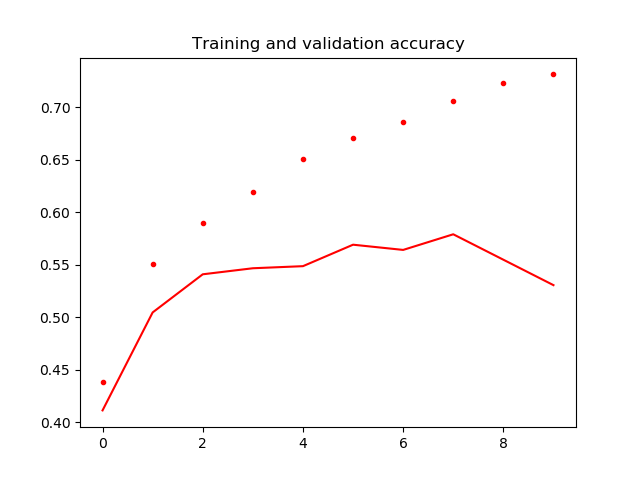
\includegraphics[width=\linewidth]{images/Setting10.png}
            \caption{Setting 10 Training and Validation Accuracy}
            \label{fig:train10}
        \end{figure}
        \paragraph{}
        The model that was found to be the best was named “Setting 15”, and had the following performance results for the training process.
        \begin{center}
        \begin{tabular}{ |c|c| } 
         \hline
         Training Accuracy & 95.61\%\\
         Validation Accuracy & 62.74\%\\
         \hline
        \end{tabular}
        \end{center}
        \paragraph{}
        The following tests results were produced, with the test images made up of samples of the warehouse photos dataset. Top 1 accuracy means that the correct class was predicted, while top 8 accuracy means that the actual class fell within the top 8 predicted classes.
        \begin{center}
        \begin{tabular}{ |c|c| } 
         \hline
         Top 1 Accuracy & 95.61\%\\
         Top 4 Accuracy & 63.33\%\\
         Top 8 Accuracy & 78.33\%\\
         \hline
        \end{tabular}
        \end{center}
        \paragraph{}
        In the graph below (Figure 12), ranked predictions refer to the percentage of classes predicted between 2nd and 8th, while unranked predictions refer to the percentage of classes outside the top 8 predictions.
        \begin{figure}[H]
            \includegraphics[width=\linewidth]{images/chart1.png}
            \caption{Setting 15 Test Accuracy}
            \label{fig:test15}
        \end{figure}
        
        \paragraph{4. MobileNet model with scraped dataset}
        Although the “Setting 15” model had a successful training period and an improved test accuracy, generalization was still not good enough to be used. Another problem was the large size of the model (166 MB), which made it difficult to deploy and slow when loading into memory.
        \paragraph{}
        A solution to this was to train a model using a different base architecture. The MobileNet architecture is different to the Inception v3 architecture in that it is designed to be small and less resource intensive. The Inception v3 network is designed for pure accuracy, and thus requires a large dataset, processing power, and training time, all of which was not available to the team.
        \paragraph{}
        Transfer learning was used once again to build a model called “Setting 16”, this time with the MobileNet base. The results for this model were very similar to “Setting 15” in terms of training results, as can be seen below.
        \begin{center}
        \begin{tabular}{ |c|c| } 
         \hline
         Training Accuracy & 93.89\%\\
         Validation Accuracy & 63.59\%\\
         \hline
        \end{tabular}
        \end{center}
        \paragraph{}
        Test results dropped off a bit from “Setting 15”, although this tradeoff in favour of prediction speed and model availability was considered to be worthwhile.
        \begin{center}
        \begin{tabular}{ |c|c| } 
         \hline
         Top 1 Accuracy & 38.33\%\\
         Top 4 Accuracy & 58.33\%\\
         Top 8 Accuracy & 65.00\%\\
         \hline
        \end{tabular}
        \end{center}
        
        \paragraph{5. New scraped dataset}
        After deploying the “Setting 16” model on the app, feedback was received with regards to the prediction performance and accuracy. Although performance was generally considered to be good and usable, the accuracy for certain classes were still poor.
        \paragraph{}
        To solve this problem, each of the classes and their respective test accuracy were inspected. It was found that classes such as “safety gloves” and “cutting disc”, which were distinct from any other classes, were consistently predicted accurately. Sets of classes that were very similar, such as “air quick coupler” and “female quick coupler”, had really poor accuracy. It was found that these sets had many overlapping images, as was verified by Google Images’ search results.
        \paragraph{}
        It became clear that a new dataset was required with a new list of classes. These classes had to be distinct enough so that there were few overlapping images, but still specific enough for example to distinguish between a countersunk screw, a self-tapping screw, and a cheesehead screw. The classes were also specifically hand-picked from Bramhope’s (the client’s) online catalogue, so that there was a direct correlation to the application domain.
        \paragraph{}
        A new model was trained with the MobileNet base, called “Setting 17”. The model had improved training results over “Setting 16”, as can be seen below.
        \begin{center}
        \begin{tabular}{ |c|c| } 
         \hline
         Training Accuracy & 92.63\%\\
         Validation Accuracy & 74.02\%\\
         \hline
        \end{tabular}
        \end{center}
        \paragraph{}
        Testing and generalization is to be conducted once a set of test images are collected. Initial testing for existing test images indicates outstanding results.
\end{document}